\documentclass{article}

\usepackage{siunitx} % Provides the \SI{}{} and \si{} command for typesetting SI units
\usepackage{graphicx} % Required for the inclusion of images
\usepackage{amsmath} % Required for some math elements 
\usepackage[export]{adjustbox} % loads also graphicx
\usepackage{listings}
\usepackage{matlab-prettifier}
\usepackage{float}
\usepackage[most]{tcolorbox}
\usepackage{amsfonts}
\usepackage{color}
\usepackage{titlesec}
\usepackage{caption}
\usepackage{subcaption}

\newcommand{\R}{\mathbb{R}}

\usepackage{xcolor}

\DeclareCaptionFont{white}{\color{white}}
\DeclareCaptionFormat{listing}{%
  \parbox{\textwidth}{\colorbox{gray}{\parbox{\textwidth}{#1#2#3}}\vskip-4pt}}
\captionsetup[lstlisting]{format=listing,labelfont=white,textfont=white}
\lstset{frame=lrb,xleftmargin=\fboxsep,xrightmargin=-\fboxsep}
\titleformat{\section}[runin]
  {\normalfont\Large\bfseries}{\thesection}{1em}{}
\titleformat{\subsection}[runin]
  {\normalfont\large\bfseries}{\thesubsection}{1em}{}


\setlength\parindent{0pt} % Removes all indentation from paragraphs

\renewcommand{\labelenumi}{\alph{enumi}.} % Make numbering in the enumerate environment by letter rather than number (e.g. section 6)

%\usepackage{times} % Uncomment to use the Times New Roman font

%----------------------------------------------------------------------------------------
%	DOCUMENT INFORMATION
%----------------------------------------------------------------------------------------

\title{AMATH 353: Homework 9 \\Due May, 4 2018 \\ ID: 1064712} % Title

\author{Trent \textsc{Yarosevich}} % Author name

\date{\today} % Date for the report

\begin{document}
\maketitle % Insert the title, author and date
\setlength\parindent{1cm}

\begin{center}
\begin{tabular}{l r}
%Date Performed: December 1, 2017 \\ % Date the experiment was performed
Instructor: Jeremy Upsal % Instructor/supervisor
\end{tabular}
\end{center}

% If you wish to include an abstract, uncomment the lines below
% \begin{abstract}
% Abstract text
% \end{abstract}

%----------------------------------------------------------------------------------------
%	SECTION 1
%----------------------------------------------------------------------------------------
\section*{Part 1}
\subsection*{a.)}
We are asked to compute the integral $\int_a^b x\cos(\frac{n\pi x}{2})$. I will also show my work here for $\int_a^b (2-x)\cos(\frac{n\pi x}{2})$ as this is how I computed the $a_n$ term later on. Starting with the first one, using division by parts we have:
\begin{equation}
\begin{aligned}
\int x\cos(\frac{n\pi x}{2}) = \int udv\\
u = x \; , \; du = dx\\
dv = \cos(\frac{n\pi x}{2})dx\\
v = \int dv = \frac{2}{n\pi}\sin(\frac{n\pi x}{2})\\
\int udv = uv - \int vdu = \frac{2x}{n\pi}\sin(\frac{n\pi x}{2}) + \frac{4}{n^2\pi^2}\cos(\frac{n\pi x}{2})
\end{aligned}
\end{equation}
\begin{tcolorbox}[minipage,colback=white,arc=0pt,outer arc=0pt]
\begin{multline}
\int_a^b x\cos(\frac{n\pi x}{2}) = \\ \frac{2b}{n\pi}\sin(\frac{n\pi b}{2}) + \frac{4}{n^2\pi^2}\cos(\frac{n\pi b}{2}) - \frac{2a}{n\pi}\sin(\frac{n\pi a}{2}) - \frac{4}{n^2\pi^2}\cos(\frac{n\pi a}{2})
\end{multline}
\end{tcolorbox}
And now the same for $\int_a^b (2-x)\cos(\frac{n\pi x}{2})$. Note that I did the definite integral directly here, unlike the previous equation.
\begin{equation}
\begin{aligned}
\int_a^b (2-x)cos(\frac{n\pi x}{2}) = \int_a^b udv\\
u = 2-x  \; , \; du = -dx\\
dv = cos(\frac{n\pi x}{2})dx\\
v = \int dv = \frac{2}{n\pi}\sin(\frac{n\pi x}{2})\\
\int vdu = \frac{4}{n^2\pi^2}\cos(\frac{n\pi x}{2})
\end{aligned}
\end{equation}
\begin{tcolorbox}[minipage,colback=white,arc=0pt,outer arc=0pt]
\begin{multline}
uv\Big|_a^b - \int_a^b vdu = \\ (2-b)\frac{2}{n\pi}\sin(\frac{n\pi b}{2}) - (2-a)\frac{2}{n\pi}\sin(\frac{n\pi a}{2}) - \frac{4}{n^2\pi^2}\cos(\frac{n\pi b}{2}) + \frac{4}{n^2\pi^2}\cos(\frac{n\pi a}{2})
\end{multline}
\end{tcolorbox}
\subsection*{b.)}
\begin{equation}
b_n = \frac{1}{2} \int_{-2}^2 f_e(x)\sin(\frac{n\pi x}{2})dx
\end{equation}
Because $f_e(x)$ is defined as the even extension of $f(x)$, and because sine is an odd function, their product is odd. Any integral of an odd function across a symmetrical domain including the origin is equal to zero, and thus $b_n = 0$.
\subsection*{c.)}
To find $a_0$ I use the following equation, which we derived in class and which results from the fact that the average value of $\sin$ and $\cos$ are both $0$:
\begin{equation}
\frac{a_0}{2} = A = \frac{1}{4}\int_{-2}^2 f_e(x)dx
\end{equation}
Because $f_e(x)$ is defined as the even extension of $f(x)$, and because the resulting domain is defined equivalently in both $f_e(x)$ and $f(x)$, we get the following:
\begin{equation}
\frac{a_0}{2} = A = \frac{1}{4}\int_{-2}^2 f_e(x)dx = 2(\frac{1}{4})\int_0^2 f_e(x)dx = \frac{1}{2}\int_0^2f(x)dx
\end{equation}
This definite integral is then evaluated for the piece-wise function with an integration constant of 0.
\begin{equation}
\begin{aligned}
A = \frac{1}{2}\Big[(\frac{1}{2}x^2) \Big|_0^1 + (2x-\frac{1}{2}x^2)\Big|_1^2\Big]\\
A = \frac{1}{2}
\end{aligned}
\end{equation}
\begin{tcolorbox}[minipage,colback=white,arc=0pt,outer arc=0pt]
\begin{equation}
a_0 = 2A = 1
\end{equation}
\end{tcolorbox}
\subsection*{d.)}
To find $a_n$ we use the following equation
\begin{equation}
a_n = \frac{1}{2} \int_{-2}^2 f_e(x)\cos(\frac{n\pi x}{2})dx
\end{equation}
taking note that the product of two even functions, $f_e(x)$ and $\cos$, is also an even function, and that the resulting domain is equivalent in both $f_e(x)$ and $f(x)$, we get the following:
\begin{equation}
a_n = \frac{1}{2} \int_{-2}^2 f_e(x)\cos(\frac{n\pi x}{2})dx = 2\frac{1}{2} \int_0^2 f_e(x)\cos(\frac{n\pi x}{2})dx = \int_0^2 f(x)\cos(\frac{n\pi x}{2})dx
\end{equation}
Because $f(x)$ is a piecewise function (shown below), the integral in this domain is defined as follows:
\[f(x)=
  \begin{cases}
			x, \; \; \; 0<x\leq 1, \\
			2-x, \; \; \; 1 < x \leq 2
            \end{cases}
\]
\begin{equation}
 \int_0^2 f(x)\cos(\frac{n\pi x}{2})dx = \int_0^1 x\cos(\frac{n\pi x}{2})dx + \int_1^2 (2-x)cos(\frac{n\pi x}{2})dx
\end{equation}
Then plugging this into the results of part a.), equations (2) and (4) above, we have the following:
\begin{multline}
a_n = \\ \Big[ \frac{2}{n\pi}\sin(\frac{n\pi}{2}) + \frac{4}{n^2\pi^2}\cos(\frac{n\pi}{2}) - 0 - \frac{4}{n^2\pi^2}\cos(0) \Big] \\ + \Big[ 0 - (1)(\frac{2}{n\pi}\sin(\frac{n\pi}{2}) - \frac{4}{n^2\pi^2}\cos(n\pi) + \frac{4}{n^2\pi^2}\cos(\frac{n\pi}{2}) \Big]
\end{multline}
By carrying out the addition and subtraction of sine/cosine terms with the same arguments, and using the equivalence $cos(n\pi) = (-1)^2$ we get:
\begin{tcolorbox}[minipage,colback=white,arc=0pt,outer arc=0pt]
\begin{equation}
a_n = \frac{8\cos(\frac{n\pi}{2}) - 4(-1)^n - 4}{n^2\pi^2}
\end{equation}
\end{tcolorbox}
\subsection*{e.)}
Now that I have my constants, I can plug them in to the following equation to plot. \textit{Please note I have uploaded the wolfram notebook I used to make these plots.} As the graphs show, $f_3$ and $f_{10}$ superficially resemble $f(x)$. As $N$ increases, we see that the fourier series is beginning to converge. In particular, comparing $f_3$ and $f_{10}$, we see the larger number of oscillations as more waves are added, but they are flattening out and more closely resembling a line. In addition, it's clear looking at the bounds that $f_{10}$ is much closer to the proper bounds of $f(0) = 0$ and $f(2) = 0$.
\begin{equation}
f(x) = \frac{a_0}{2} + \sum_{n=1}^{\infty} a_n\cos(\frac{n\pi x}{2})
\end{equation}
\begin{figure}[H]
  \centering
    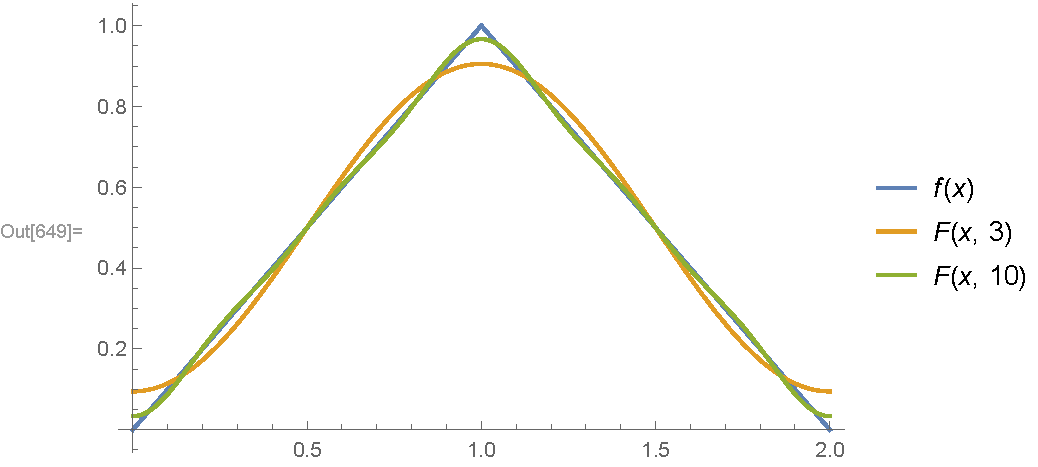
\includegraphics[width=\textwidth, scale = 1.25]{hw_9_plots.pdf}
    \caption{$f(x) \text{ and } n = 3, 10$}
\end{figure}
\end{document}